% !TeX root = RJwrapper.tex
\title{autoplotly - Automatic Generation of Interactive Visualizations for
Popular Statistical Results}
\author{by Yuan Tang}

\maketitle

\abstract{%
autoplotly is an R package that provides functionalities to
automatically generate interactive visualizations for many popular
statistical results supported by ggfortify package with plotly.js and
ggplot2 style. The generated visualizations can also be easily extended
using ggplot2 syntax while staying interactive.
}

\subsection{Introduction}\label{introduction}

Introductory section which may include references in parentheses
\citep{R}, or cite a reference such as \citet{R} in the text.

\subsection{Background}\label{background}

\subsection{Software Architecture}\label{software-architecture}

This section may contain a figure such as Figure \ref{figure:rlogo}.

\begin{figure}[htbp]
  \centering
  
\includegraphics{Rlogo}
  \caption{The logo of R.}
  \label{figure:rlogo}
\end{figure}

\subsection{Illustrations}\label{illustrations}

There will likely be several sections, perhaps including code snippets,
such as:

\begin{Schunk}
\begin{Sinput}
autoplotly(prcomp(iris[c(1, 2, 3, 4)]), data = iris, frame = TRUE, colour = 'Species')
\end{Sinput}
\end{Schunk}

\begin{figure}[htbp]
  \centering
  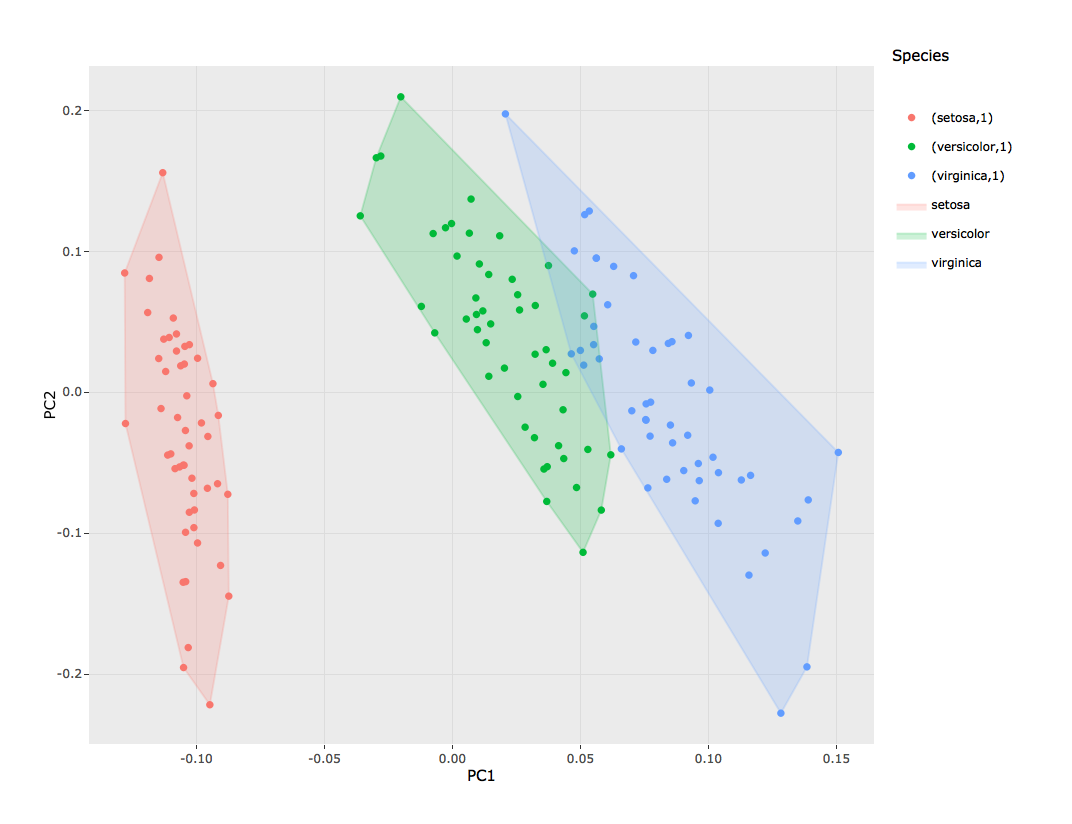
\includegraphics[width=145mm,scale=0.8]{images/iris_pca_full.png}
  \caption{PCA with clolors and boundary for each class.}
  \label{figure:pca_full}
\end{figure}

TODO: Hoverover metadata TODO: Zooming in details TODO: Extensibilty
with ggplot2 TODO: Extensibility with plotly TODO: Exportability with
export(p, ``inst/images/iris\_pca\_full.png'')

Forecasting packages such as \CRANpkg{forecast} \citep{forecast},
\CRANpkg{changepoint} \citep{changepoint}, \CRANpkg{strucchange}
\citep{strucchange}, and \CRANpkg{dlm} \citep{dlm}, are popular choices
for statisticians and researchers. Interactive visualizations of
predictions and statistical results from those packages can be generated
automatically using the functions provided by \pkg{autoplotly} with the
help of \pkg{ggfortify}.

The \pkg{autoplotly} function automatically plots the change points with
optimal positioning for the \code{AirPassengers} data set found in the
\pkg{changepoint} package using the \code{cpt.meanvar} function, shown
in Figure \ref{figure:changepoint_caption}.

\begin{Schunk}
\begin{Sinput}
library(changepoint)
autoplotly(cpt.meanvar(AirPassengers))
\end{Sinput}
\end{Schunk}

\begin{figure}[htbp]
  \centering
  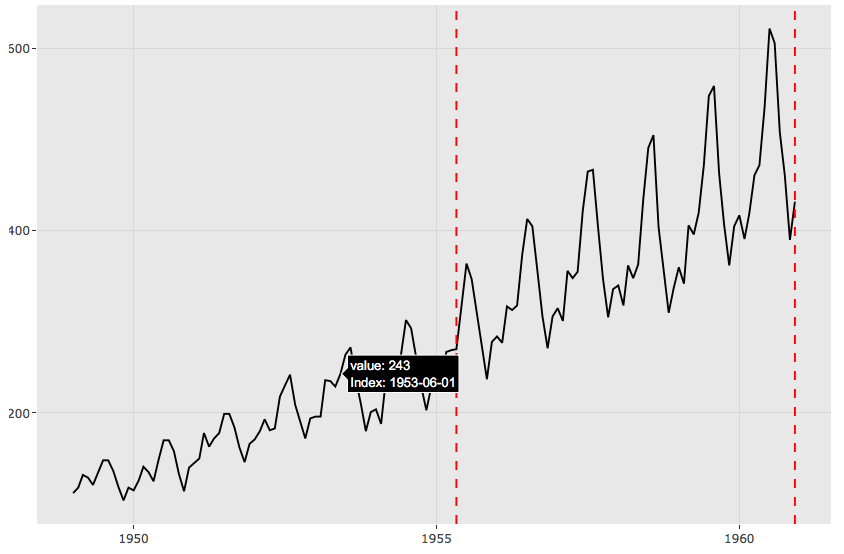
\includegraphics[width=145mm,scale=0.8]{images/changepoint_caption.png}
  \caption{Change points with optimal positioning for AirPassengers.}
  \label{figure:changepoint_caption}
\end{figure}

The \pkg{autoplotly} function automatically plots the original and
smoothed line from Kalman filter function in \pkg{dlm} package as shown
in Figure \ref{figure:dlm_caption}.

\begin{Schunk}
\begin{Sinput}
library(dlm)
form <- function(theta){
  dlmModPoly(order = 1, dV = exp(theta[1]), dW = exp(theta[2]))
}
model <- form(dlmMLE(Nile, parm = c(1, 1), form)$par)
filtered <- dlmFilter(Nile, model)
autoplotly(filtered)
\end{Sinput}
\end{Schunk}

\begin{figure}[htbp]
  \centering
  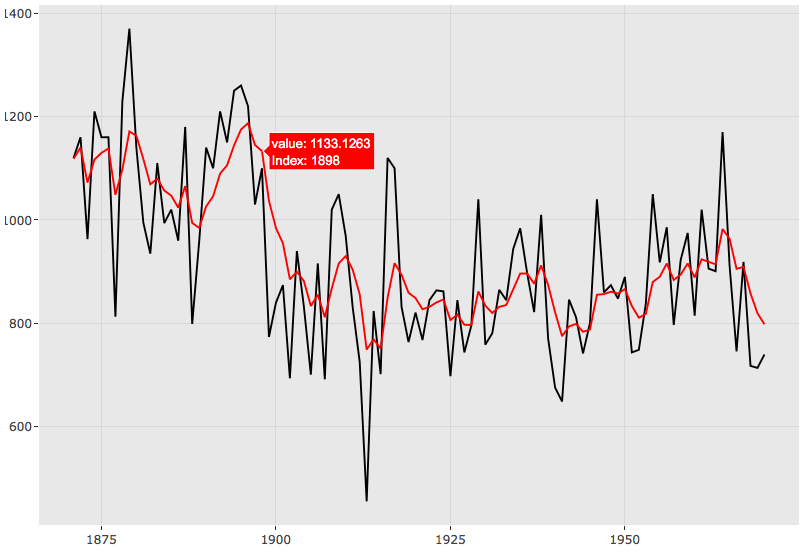
\includegraphics[width=145mm,scale=0.8]{images/dlm_caption.png}
  \caption{Smoothed time series by Kalman filter.}
  \label{figure:dlm_caption}
\end{figure}

Additionally, \pkg{autoplotly} plots the optimal break points where possible structural changes happen in the regression models built by the \code{strucchange::breakpoints}, shown in Figure \ref{figure:strucchange_caption}.

\begin{Schunk}
\begin{Sinput}
library(strucchange)
autoplotly(breakpoints(Nile ~ 1), ts.colour = "blue", ts.linetype = "dashed",
           cpt.colour = "dodgerblue3", cpt.linetype = "solid")
\end{Sinput}
\end{Schunk}

\begin{figure}[htbp]
  \centering
  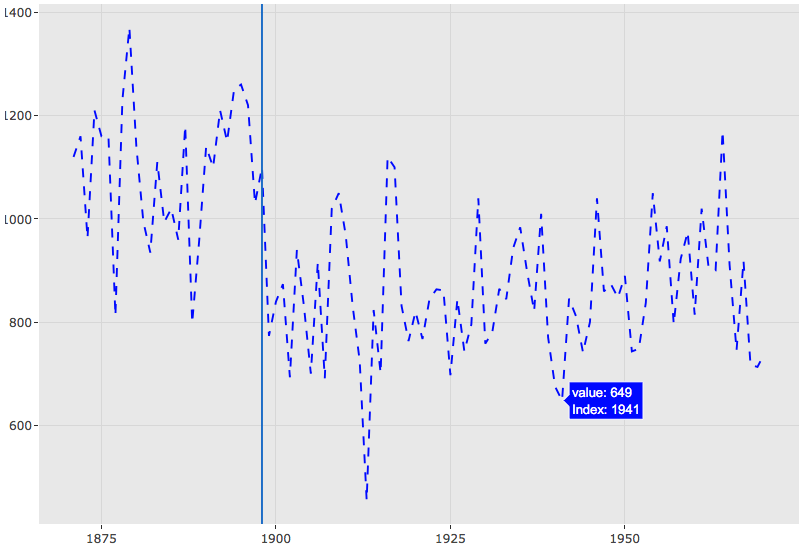
\includegraphics[width=145mm,scale=0.8]{images/strucchange_caption.png}
  \caption{Optimal break points with possible structural changes.}
  \label{figure:strucchange_caption}
\end{figure}


The \code{autoplotly} can also automatically generate interactive plots for results producuced by \pkg{splines}, shown in Figure \ref{figure:splines_caption}

\begin{Schunk}
\begin{Sinput}
library(splines)
autoplotly(ns(diamonds$price, df = 6))
\end{Sinput}
\end{Schunk}

\begin{figure}[htbp]
  \centering
  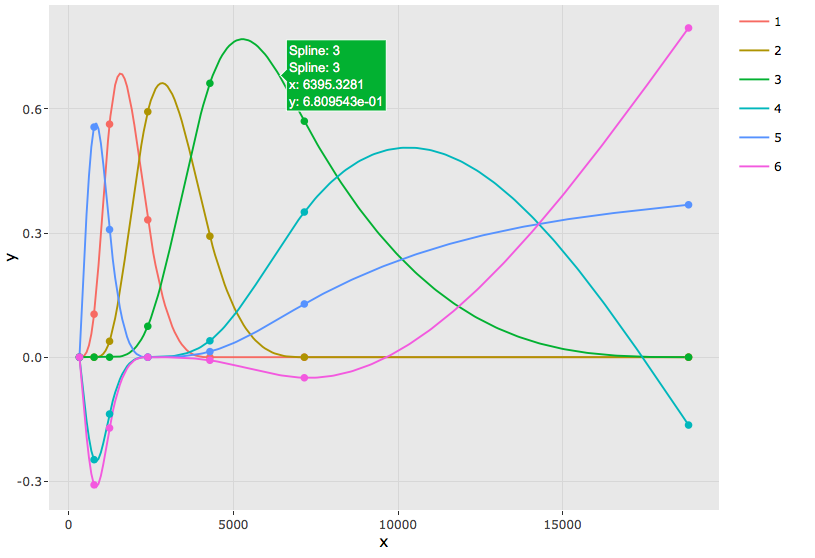
\includegraphics[width=145mm,scale=0.8]{images/splines_caption.png}
  \caption{B-spline basis points for natural cubic spline with boundary knots.}
  \label{figure:splines_caption}
\end{figure}

\subsection{Summary}\label{summary}

This file is only a basic article template. For full details of
\emph{The R Journal} style and information on how to prepare your
article for submission, see the
\href{https://journal.r-project.org/share/author-guide.pdf}{Instructions
for Authors}. \bibliography{RJreferences}

\address{%
Yuan Tang\\
H2O.ai\\
2309 Wake Robin Drive\\ West Lafayette, IN 47906\\
}
\href{mailto:terrytangyuan@gmail.com}{\nolinkurl{terrytangyuan@gmail.com}}

